%!TEX root = ../../../adrien_gomar_phd.tex

\subsection{Geometry}
\label{sub:cror_geometry}

Figure~\ref{fig:cror_geometry} depicts the main
geometrical parameters of a CROR.
It is composed of two rotors, the first one is called
the front rotor and the second one is called the rear or aft rotor.
Generally, they do not have the same diameter $D$ and rotation speed
$\Omega$. Thus, subscript $F$ and $R$ denotes respectively,
the front and the rear parameter. The diameter is expressed in meters
while the rotation speed is expressed in radians per seconds.
As the rotors are contra-rotating, their rotation speed is opposed.
The difference of diameter is called the clipping or cropping
of the blades and is evaluated through the non-dimensional parameter
$\kappa$:
\begin{equation}
    \kappa = \frac{D_F - D_R}{D_F}.
\end{equation}
This clipping is done to avoid the interaction 
with the rear rotor of the tip vortex shed
by the front rotor. In fact, by clipping the rear
rotor, tip vortex of th front rotor is not likely
to hit the rear rotor.
Finally, the spacing between the rotors
is evaluated as the difference between the axial minimum of the
rear blade minus the maximum of the front blade. The spacing
is one of the adjustment parameters used to minimize the unsteady
interaction between the rotors to reduce noise.
\begin{figure}[htbp]
  \centering
  \includegraphics*[scale=0.3]{cror_geometry.pdf}
  \caption{Contra-rotating open rotor geometrical parameters.}
  \label{fig:cror_geometry}
\end{figure}

The contra-rotating open rotor architecture is composed of a classical engine
turbomachinery whose fan is not within a nacelle. As explain
above, this help increasing the mass-flow of the primary flow
which leads to a higher propulsive efficiency.
Two main architectures are retained. One based on a gearbox, the second
being build around a statorless low-pressure turbine.
\begin{figure}[htb]
  \centering
  \subfigure[Geared design]{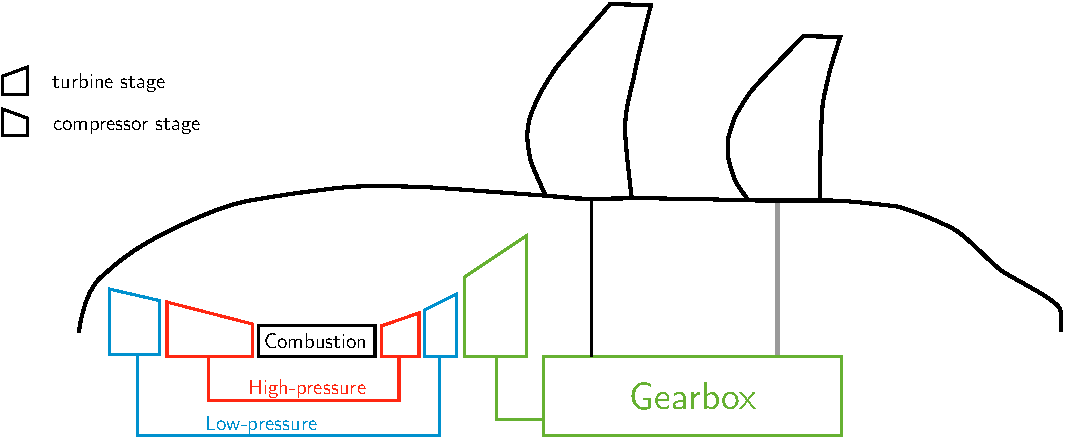
\includegraphics[width=.4\textwidth]{geared_cror.pdf}}
  \subfigure[Statorless low-pressure turbine design]{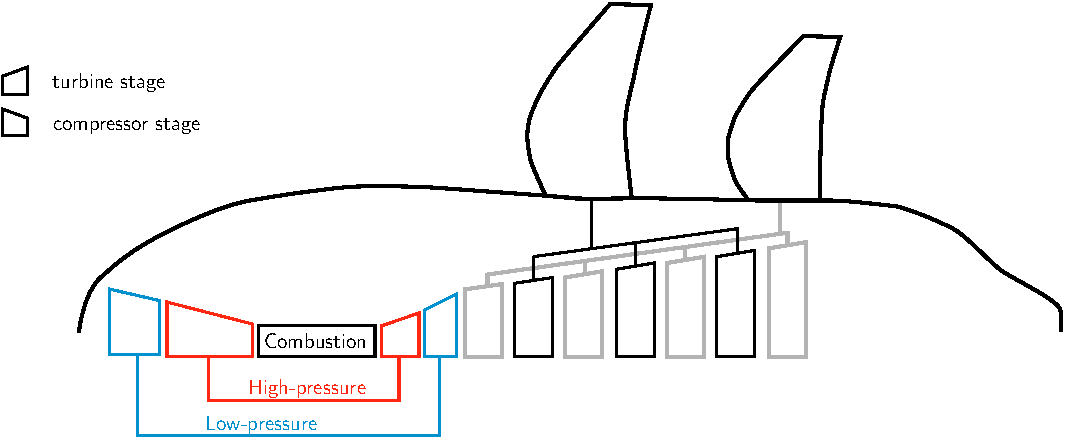
\includegraphics[width=.4\textwidth]{stator_less_cror.pdf}}
  \caption{Contra-rotating open rotor architectures.}
  \label{fig:cror_architectures}
\end{figure}

\subsection{Velocity triangle}
\label{sub:cror_velocity_triangle}

The basic idea behind the CROR concept is that a propeller has a 
better propulsive efficiency than a turbofan. However,
a residual tangential velocity is present behind a propeller, that limits
the benefit of such a configuration.
In fact, from the application of the velocity triangle to a propeller configuration
as shown in Fig.~\ref{fig:cror_velocity_triangle_propeller}, one can
observe that the outlet velocity (noted $V^{out}_x$) is not axial
yielding a residual tangential velocity $\Delta V_{\theta}$. This tangential velocity forms
the swirl observed behind a propeller. First, this is a lost energy and
second, it produces a torque that has an impact on the flight dynamics
of the aircraft. To alleviate this effect, one can use two propellers
that are counter-rotating as for instance the TP$400$ propellers
in the Airbus-A$400$M military airplane but this does not recover
the swirl energy that is lost.

To recover this lost energy, a second contra-rotating rotor can be used.
\begin{figure}[htbp]
  \centering
  \includegraphics*[scale=0.40]{velocity_triangle_cror.pdf}
  \caption{Velocity triangle applied to a contra-rotating open rotor configuration.}
  \label{fig:velocity_triangle_cror}
\end{figure}
Figure~\ref{fig:velocity_triangle_cror} shows the application
of the velocity triangle to a CROR configuration. The swirl
energy that was lost in the propeller is now used to 
produce more thrust. Thus, a CROR has a better propulsive
efficiency than a propeller, which explains its study as
a greener engine. \citet{Strack1981} and \citet{Hager1988} showed that
using a contra-rotating open rotor technology over
a single propeller gave an increase of $6-8\%$
of propulsive efficiency, explaining its regained of interest.

\subsection{Similarity coefficients}
\label{sub:cror_similarity_coeff}

In the case of a CROR configuration, two rotors are considered.
Two main ways exists to evaluate the global value of the
similarity coefficients. The first one, chosen by
\citet{Bechet2011} among others, is to consider
that the non-dimensioning parameter $D$, $n$ and $J$ are those
of the front rotor for both rotors:
\begin{equation}
    J_F = J_R = \frac{V_0}{n_F D_F}, \quad
    C_t = \frac{F_{x_F} + F_{x_R}}{\rho_F n_F ^ 2  D_F ^ 4}, \quad
    C_p = \Omega_F \frac{M_{x_F} + M_{x_R}}{\rho_F n_F ^ 3 D_F ^ 5}, \quad
    \eta = J_F \frac{C_t}{C_p}.
\end{equation} 
The second one uses the non-dimensioning parameter of the current rotor,
as done by \citet{Stuermer2008} and \citet{Zachariadis2011}:
\begin{equation}
    \begin{split}
        J_F = \frac{V_0}{n_F D_F}, \quad
        C_{t_F} = \frac{F_{x_F}}{\rho_F n_F ^ 2  D_F ^ 4}, \quad
        C_{p_F} = \frac{M_{x_F}\Omega_F}{\rho_F n_F ^ 3 D_F ^ 5}, \quad
        \eta_F = J_F \frac{C_{t_F}}{C_{p_F}} \\
        J_R = \frac{V_0}{n_R D_R}, \quad
        C_{t_R} = \frac{F_{x_R}}{\rho_R n_R ^ 2  D_R ^ 4}, \quad
        C_{p_R} = \frac{M_{x_R}\Omega_F}{\rho_R n_R ^ 3 D_R ^ 5}, \quad
        \eta_R = J_R \frac{C_{t_R}}{C_{p_R}}.
    \end{split}
\end{equation} 
The traction and power coefficients of the rear rotor are
computed using their own advance ratio, diameter and rotation frequency.
However, computing the advance ratio of the rear rotor is tedious, as
the free-stream velocity should be updated to take into account
for the acceleration generated by the front rotor. Nevertheless, the free-stream
velocity is chosen to be $V_0$ for both rotors, which is of course not true.
Finally, the efficiency is then computed rotor per rotor and
assembled through an arithmetic summation:
\begin{equation}
    \eta = \frac{J_F C_{t_F} + J_R C_{t_R}}{C_{p_F} + C_{p_R}}.
\end{equation}
This is the approach retained in this thesis.
